\section{Methodology}

\begin{figure}[h!]
  \centering 
    \includegraphics[width=0.98\linewidth]{figs/overview}
  \caption{Overview of the 3D anomaly detection pipeline.}
  \label{fig:overview}
\end{figure}

Given an input point cloud \(\mathcal{P} = \{\mathbf{p}_i \in \mathbb{R}^3\}_{i=1}^N\), the proposed framework leverages a frozen pre-trained point-cloud Transformer and a small set of lightweight trainable adapters to obtain spatially coherent and anomaly-sensitive representations. The Transformer backbone consists of \(L\) encoder layers, each producing \(M\) patch tokens of dimension \(D\). We denote the patch-token matrix and class token at Transformer layer \(i\) as \(\mathbf{T}_i \in \mathbb{R}^{M\times D}\) and \(c_i \in \mathbb{R}^{1\times D}\), respectively. Collectively, the hierarchical token set is \(\mathbf{T} = \{\mathbf{T}_1, \dots, \mathbf{T}_L\}\) with a total of \(T = L\cdot M\) tokens. Our goal is to transform these unordered layer-wise tokens into a semantically ordered sequence \(\mathbf{T}_{\mathrm{ord}}\in\mathbb{R}^{T\times D}\) via the proposed \textbf{Geometric Semantic-Aware Sorter (GSAS)}, fuse them using a state-space adapter (Mamba) to produce enriched contextual features \(y_{1:T}\in\mathbb{R}^{T\times D}\), and finally apply a lightweight attention-based discriminator for per-patch anomaly localization. To maintain parameter efficiency, all Transformer weights remain frozen; only the GSAS, Mamba adapters, the selective anomalous feature generator, and the cross-patch attention discriminator are trainable.

\subsection{Backbone}

Local patch extraction is performed once per input cloud and the resulting patch identities are preserved across Transformer layers. Specifically, we apply Farthest Point Sampling (FPS) to select \(M\) patch centers \(\{p_j\in\mathbb{R}^3\}_{j=1}^M\) (indices \(j\) refer to patch centers), and for each center we collect a fixed-size local neighborhood via \(K\)-nearest neighbors (KNN). Each neighborhood is embedded by a lightweight PointNet encoder followed by a small positional-encoding MLP to produce an initial patch embedding \(x_j^{(0)}\in\mathbb{R}^D\). These \(M\) patch embeddings (plus a global class token) are then fed into the frozen Point-MAE Transformer~\cite{pang2022masked} pre-trained on ShapeNet~\cite{chang2015shapenet}. Formally, the \(i\)-th Transformer block \(\ell_i(\cdot)\) computes
\begin{equation}
[c_i;\,\mathbf{T}_i] \;=\; \ell_i([c_{i-1};\,\mathbf{T}_{i-1}]), \qquad i=1,\dots,L,
\end{equation}
where \(\mathbf{T}_i = [t_{i,1};\dots;t_{i,M}]\in\mathbb{R}^{M\times D}\) and \(c_i\in\mathbb{R}^{1\times D}\). Importantly, the spatial coordinates \(\{p_j\}\) (the patch centers) are associated with the corresponding patch index \(j\) and are reused for all Transformer layers, so that token \(t_{i,j}\) at layer \(i\) corresponds to the same geometric patch center \(p_j\).

\subsection{Geometric Semantic-Aware Sorter (GSAS)}
\label{sec:gsas}

\begin{figure}[h!]
  \centering 
    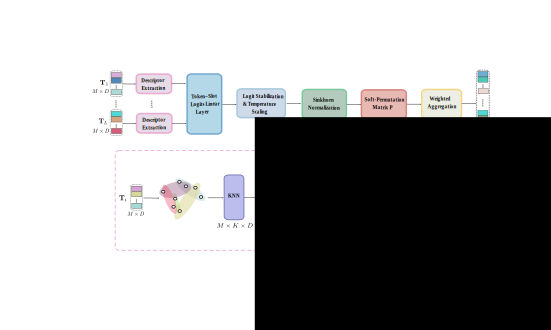
\includegraphics[width=0.98\linewidth]{figs/GSAS}
  \caption{GSAS.}
  \label{fig:GSAS}
\end{figure}

Point clouds admit no canonical linear ordering in \(\mathbb{R}^3\); nevertheless, sequence models (e.g., state-space architectures) require an ordered input. The Geometric Semantic-Aware Sorter (GSAS) produces a differentiable, geometry- and semantics-aware ordering of the full set of Transformer patch tokens such that the resulting ordered sequence preserves local surface adjacency and semantic affinity while remaining end-to-end trainable. Below we give a precise, dimensionally consistent description of GSAS and the auxiliary regularizers that prevent degenerate assignments.

We assume patch extraction (FPS + KNN) is performed once per input cloud and that the resulting \(M\) unique patch centers \(\{p_j\in\mathbb{R}^3\}_{j=1}^M\) are reused across Transformer layers. The frozen Transformer produces per-layer patch tokens \(t_{i,j}\in\mathbb{R}^D\) for layer \(i\in\{1,\dots,L\}\) and patch index \(j\in\{1,\dots,M\}\). We enumerate the full set of \(T=L\cdot M\) tokens with a single global index \(t\in\{1,\dots,T\}\) via a bijection \((i,j)\mapsto t\) (and denote the inverse mappings \(i(t), j(t)\) when needed). The patch center associated with global token \(t\) is therefore \(p_{j(t)}\) (and we may write \(p_t\) as shorthand, noting \(p_t = p_{j(t)}\)). GSAS maps the unordered set \(\{t_{i,j}\}\) to an ordered sequence \(\mathbf{T}_{\mathrm{ord}}\in\mathbb{R}^{T\times D}\) using a differentiable soft-permutation matrix \(P\in[0,1]^{T\times T}\) (rows = tokens, columns = ordered slots).

\paragraph{Permutation-invariant local descriptors (graph-on-patches, within-layer aggregation).}
Construct a kNN graph on the unique patch centers \(\{p_j\}_{j=1}^M\); denote the neighbor set of patch \(j\) by \(\mathcal{N}_{\mathrm{patch}}(j)\subset\{1,\dots,M\}\). For a given token \(t\) corresponding to \((i,j)\) (i.e., \(i=i(t), j=j(t)\)), we compute a permutation-invariant local descriptor by aggregating features from the same Transformer layer \(i\) of neighboring patches (i.e., tokens \(t_{i,u}\) for \(u\in\mathcal{N}_{\mathrm{patch}}(j)\)). Explicitly:
\begin{equation}
u_{i,j} \;=\; \mathrm{MaxPool}\Big(\big\{\,W_{\downarrow}\,t_{i,u} + b_{\downarrow} \ \big|\ u\in\mathcal{N}_{\mathrm{patch}}(j)\big\}\Big)\in\mathbb{R}^{d_a},
\end{equation}
where \(t_{i,u}\in\mathbb{R}^D\) is the token at layer \(i\) of neighbor patch \(u\), \(W_{\downarrow}\in\mathbb{R}^{d_a\times D}\), \(b_{\downarrow}\in\mathbb{R}^{d_a}\), and the MaxPool is element-wise across the neighbor set. Using the bijection \((i,j)\!\mapsto\! t\) we set \(E_{t,:}=u_{i(t),j(t)}\) to collect descriptors into \(E\in\mathbb{R}^{T\times d_a}\).

\paragraph{Token-slot affinities and differentiable soft-permutation.}
We set the number of ordered slots equal to the total token count, \(S_{\mathrm{slots}}=T\). The raw token-slot logits (affinities) are computed as
\begin{equation}
\mathbf{G} \;=\; E\,W_{\uparrow} + \mathbf{1}\,b_{\uparrow}^\top \in\mathbb{R}^{T\times T},
\end{equation}
where \(W_{\uparrow}\in\mathbb{R}^{d_a\times T}\), \(b_{\uparrow}\in\mathbb{R}^T\), and \(\mathbf{1}\in\mathbb{R}^{T\times 1}\) is an all-ones column. Entry \(\mathbf{G}_{t,s}\) is the unnormalized affinity of token \(t\) to ordered slot \(s\).

To obtain a differentiable approximately-permutation matrix we apply temperature-scaled exponentiation followed by the Sinkhorn operator. For numeric stability subtract the column-wise maximum before exponentiation: let \(v\in\mathbb{R}^T\) be the vector with entries \(v_s=\max_{t}\mathbf{G}_{t,s}\). Then
\begin{equation}
\tilde{\mathbf{G}} \;=\; (\mathbf{G} - \mathbf{1}\,v^\top)/\tau \in\mathbb{R}^{T\times T},
\quad\text{and}\quad
P \;=\; \mathrm{Sinkhorn}\big(\exp(\tilde{\mathbf{G}}),\,K_{\mathrm{sink}}\big)\in[0,1]^{T\times T},
\end{equation}
where \(\tau>0\) is a temperature (smaller \(\tau\) yields sharper assignments) and \(\mathrm{Sinkhorn}(\cdot,K_{\mathrm{sink}})\) denotes \(K_{\mathrm{sink}}\) iterations of alternating row- and column-normalization producing an (approximately) doubly-stochastic matrix. During training this soft-permutation is differentiable; at inference time one may optionally discretize \(P\) (e.g., via the Hungarian algorithm on \(-\mathbf{G}\)) if a hard permutation is required.

\paragraph{Weighted aggregation into ordered slots.}
Given the token feature matrix \(X\in\mathbb{R}^{T\times D}\) with rows \(X_t=t_{i(t),j(t)}\), the ordered-token matrix is obtained by weighted aggregation into slots:
\begin{equation}
\mathbf{T}_{\mathrm{ord}} \;=\; P^\top X \in\mathbb{R}^{T\times D},\qquad
\mathbf{T}_{\mathrm{ord}}[s,:]=\sum_{t=1}^T P_{t,s}\,X_t.
\end{equation}
Because \(P\) is (approximately) doubly-stochastic, this yields one feature vector per ordered slot; the weighted aggregation is differentiable so gradients propagate to all GSAS parameters \(W_{\downarrow},b_{\downarrow},W_{\uparrow},b_{\uparrow}\).

\paragraph{Auxiliary regularizers for locality and assignment sharpness.}
To avoid degenerate (diffuse or collapsed) assignments and to encourage geometric locality in the induced order we add two auxiliary regularizers.

\textbf{Entropy penalty.} A column-wise entropy penalty discourages diffuse assignments into a given slot:
\begin{equation}
\mathcal{L}_{\mathrm{ent}} \;=\; \frac{1}{T}\sum_{s=1}^T H(P_{:,s}),\qquad
H(\pi)=-\sum_{t}\pi_t\log(\pi_t+\epsilon_{\mathrm{ent}}),
\end{equation}
where \(\epsilon_{\mathrm{ent}}>0\) is a small constant for numerical stability (and the natural logarithm is used). This term encourages each slot to receive a concentrated assignment.

\textbf{Locality penalty (normalized).} Let \(\tilde s = \dfrac{s-1}{\max(1,T-1)}\in[0,1]\) denote the normalized slot coordinate (so slot positions are scale-invariant to \(T\) and safely defined when \(T=1\)), and define the expected (normalized) slot index for token \(t\) as
\begin{equation}
\mu_t \;=\; \sum_{s=1}^T \tilde s\, P_{t,s} \in [0,1].
\end{equation}
Denote by \(j(t)\) the patch index associated with token \(t\). Define a geometric affinity between patches via
\begin{equation}
w_{t,u} \;=\; \exp\!\big(-\|p_{j(t)}-p_{j(u)}\|^2/\sigma_p^2\big),
\end{equation}
where \(\sigma_p\) is a bandwidth parameter. To avoid density bias we average the locality penalty per token:
\begin{equation}
\mathcal{L}_{\mathrm{loc}} \;=\; \sum_{t=1}^T \frac{1}{\sum_{u=1}^T w_{t,u} + \epsilon_{\mathrm{norm}}}\sum_{u=1}^T w_{t,u}\,\big(\mu_t - \mu_u\big)^2,
\end{equation}
where \(\epsilon_{\mathrm{norm}}>0\) is a small constant for stability in the normalization. Because \(w_{t,u}\) depends only on the underlying patch centers \(\{p_j\}\), tokens corresponding to the same patch (different layers) naturally receive maximal affinity; if a design choice requires discounting same-patch across-layer pairs one may set \(w_{t,u}=0\) when \(j(t)=j(u)\) — otherwise the above encourages tokens from the same patch to be placed nearby in the final order.

Both \(\mathcal{L}_{\mathrm{ent}}\) and \(\mathcal{L}_{\mathrm{loc}}\) are weighted by small coefficients \(\alpha_{\mathrm{ent}},\alpha_{\mathrm{loc}}>0\) and incorporated into the overall training loss (see Sec.~\ref{sec:loss}).

\paragraph{Remarks on shapes and stability.} All shapes and operations above are dimensionally consistent: \(E\in\mathbb{R}^{T\times d_a}\), \(W_{\uparrow}\in\mathbb{R}^{d_a\times T}\) producing \(\mathbf{G}\in\mathbb{R}^{T\times T}\), \(\exp(\cdot)\) is elementwise, Sinkhorn returns \(P\in\mathbb{R}^{T\times T}\), and \(P^\top X\) yields \(\mathbf{T}_{\mathrm{ord}}\in\mathbb{R}^{T\times D}\). The kNN graph is explicitly constructed over the unique patch centers \(\{p_j\}\) (shared across layers) and neighborhood aggregation pools neighbor tokens \emph{within the same Transformer layer} by design, which enforces geometric consistency while keeping layer semantics separated during descriptor computation. For numerical stability we recommend subtracting the per-column maximum prior to exponentiation (as shown), using \(\epsilon_{\mathrm{ent}}\) inside the entropy log, and using \(\epsilon_{\mathrm{norm}}\) in the locality normalization.


\subsubsection{Mamba Feature Adapter}

After GSAS produces the ordered token matrix $\mathbf{T}_{\mathrm{ord}}\in\mathbb{R}^{T\times D}$, let the row-wise sequence be
$$
x_{1:T},\qquad x_t=\mathbf{T}_{\mathrm{ord}}[t,:]\in\mathbb{R}^D,\quad t=1,\dots,T.
$$
The Mamba adapter is formulated as a state-space model that fuses long-range, layer-wise context along the GSAS-induced ordering. Let the latent dimension be $S$. The recurrence and output equations are defined as
\begin{equation}
h_t = A\,h_{t-1} + B\,x_t,\qquad h_0=\mathbf{0}\in\mathbb{R}^S,
\end{equation}
\begin{equation}
\tilde{q}_t = C\,h_t + D\,x_t \in\mathbb{R}^D,
\end{equation}
where
$$
A\in\mathbb{R}^{S\times S},\quad 
B\in\mathbb{R}^{S\times D},\quad 
C\in\mathbb{R}^{D\times S},\quad 
D\in\mathbb{R}^{D\times D}.
$$
The sequence of adapted outputs is collected as
$$
Q=[\tilde{q}_1,\dots,\tilde{q}_T]^\top\in\mathbb{R}^{T\times D},
$$
and, for consistency with the subsequent modules, $q_t\equiv\tilde{q}_t$.

The GSAS module determines the sequence order $x_{1:T}$, while the Mamba adapter performs contextual integration along this induced order without altering the token arrangement. The parameters $\{A,B,C,D\}$ are shared across all time steps, ensuring parameter efficiency and preserving the linear computational complexity with respect to sequence length $T$. Specifically, Mamba operates in $\mathcal{O}(T)$ time and requires $\mathcal{O}(S)$ additional memory per step, in contrast to the $\mathcal{O}(T^2)$ cost of full self-attention. The residual term $D\,x_t$ maintains per-token fidelity, while $C\,h_t$ introduces long-range contextual dependencies through the recurrent hidden state. The Mamba parameters are optimized jointly with the GSAS parameters, positional MLP, anomaly-scaling $\gamma$, and discriminator weights, whereas the Transformer backbone remains frozen.

\subsection{Anomalous Feature Generator}
Industrial defects in 3D point clouds are typically sparse, subtle, and spatially localized. To simulate such defects during training without requiring external anomaly examples, we introduce a lightweight, selective feature-space perturbation that synthesizes pseudo-anomalous tokens by injecting noise into a sparse subset of adapted token embeddings. Given output from Mamba feature adapter $Y$.

We sample an independent Bernoulli mask per token to determine corruption:
\begin{equation}
m_t \sim \mathrm{Bernoulli}(p),\qquad m_t\in\{0,1\},
\end{equation}
where \(p\in(0,1)\) controls expected corruption sparsity and is selected on validation (to reflect realistic, sparse defect rates we typically choose \(p\ll 0.5\) and tune it on held-out data). When \(m_t=1\) the token is corrupted by an additive isotropic Gaussian perturbation in the canonical token space:
\begin{equation}
\varepsilon_t \sim \mathcal{N}\big(0,\sigma^2 I_D\big),
\end{equation}
where \(\sigma>0\) controls perturbation scale (we validate \(\sigma\); a practical value is \(\sigma=0.1\)). The pseudo-anomalous token is defined as
\begin{equation}
\tilde{q}_t \;=\; q_t + \gamma\, m_t\, \varepsilon_t,
\end{equation}
where \(\gamma\ge 0\) is a learnable scalar that adaptively rescales the injected perturbation (initialized to a small positive value). When \(m_t=0\) we have \(\tilde{q}_t=q_t\). This corruption mechanism is applied only during training; at inference time the generator is disabled (\(m_t\equiv 0\)) and all tokens remain clean.

The selective (sparse) corruption contrasts with indiscriminate global noise: by corrupting a small fraction of slots we emulate localized defects while preserving the normal manifold for the majority of features. Because sparse corruption can induce class imbalance, we (i) recommend validating \(p\) on held-out data and (ii) mitigate imbalance via weighted loss or controlled sampling (details in the training section).

\subsection{Cross-Patch Attention Discriminator}
Detecting defects often requires contextual comparison across patches. We therefore employ a lightweight attention-based discriminator that jointly processes all patch slots and outputs a scalar logit per slot. To preserve spatial information and to generalize across varying patch arrangements, positional embeddings are derived from patch center coordinates rather than learned per-slot indices. Let \(p_t\in\mathbb{R}^3\) denote the patch center associated with slot \(t\); the positional embedding is computed by a small coordinate MLP:
\begin{equation}
e_t \;=\; \mathrm{PE\text{-}MLP}(p_t) \in\mathbb{R}^D.
\end{equation}

During training we construct a single mixed input sequence for the discriminator in which corrupted tokens replace clean tokens in-place. The discriminator input for slot \(t\) is therefore
\begin{equation}
\hat{q}_t \;=\; \big(m_t\,\tilde{q}_t + (1-m_t)\,q_t\big) + e_t \;=\; q_t + m_t(\gamma\varepsilon_t) + e_t,
\end{equation}
and the supervision label is \(y_t=m_t\). Inference uses the same pipeline but with \(m_t\equiv 0\) so that \(\hat{q}_t=q_t+e_t\).

Let \(H\) denote the number of attention heads and \(d_{\mathrm{head}}=D/H\) the per-head dimension; in practice we choose \(D\) divisible by \(H\) or insert a thin linear projection to meet this constraint. The discriminator applies a single multi-head self-attention layer followed by a compact shared MLP head that maps each token to a scalar logit:
\begin{align}
Z \; &=\; \mathrm{MHA}(\{\hat{q}_t\}_{t=1}^T)\in\mathbb{R}^{T\times D},\\
s_t \; &=\; \mathrm{MLP}_{\mathrm{head}}(Z_t)\in\mathbb{R}.
\end{align}
Here \(\mathrm{MHA}(\cdot)\) denotes standard multi-head self-attention with appropriate query/key/value projections, scaled dot-product attention, residual connections, dropout and layer normalization; \(\mathrm{MLP}_{\mathrm{head}}\) is a two-layer feedforward network (one hidden layer) shared across slots and producing a scalar logit. Layer normalization and dropout are included to stabilize training. Because the discriminator processes all tokens jointly, each output \(s_t\) reflects both local evidence and global context, improving sensitivity to structured or context-dependent defects compared to independent per-slot scoring.

At test time the discriminator receives only clean tokens \(\{q_t\}\) augmented with positional embeddings \(e_t\) and outputs per-slot logits \(s_t\). These per-slot scores are reprojected to the original point cloud by assigning each point the maximal score of the patches that contain it (see Inference section).

\subsection{Loss Function and Training}
\label{sec:loss}

We jointly optimize the trainable components (GSAS parameters, Mamba adapter parameters, positional-embedding MLP, the anomaly-scaling \(\gamma\), and discriminator parameters) using a patch-wise binary classification objective. Let \(\Theta\) denote the set of all trainable parameters. For a training batch we accumulate \(P\) supervised token slots (summed across batch and sequence). We use a numerically-stable logits-based binary cross-entropy implemented as BCE-with-logits. The per-slot logits-based loss (stable form) is:
\begin{equation}
\ell_{\mathrm{BCElogits}}(s,y) \;=\; \max(s,0) - s\,y + \log\big(1+\exp(-|s|)\big),
\end{equation}
and the unweighted batch loss is \(\mathcal{L}_{\mathrm{BCE}}=\frac{1}{P}\sum_{t=1}^P \ell_{\mathrm{BCElogits}}(s_t,y_t)\). To mitigate class imbalance when corruption is sparse we optionally use a positive-class weighting factor \(w_+>0\) (e.g., \(w_+=(1-p)/p\) or a value tuned on validation) via the standard \texttt{pos\_weight} mechanism of BCE-with-logits; this multiplies the contribution of positive (corrupted) examples.

We complement \(\mathcal{L}_{\mathrm{BCE}}\) with the GSAS regularizers \(\mathcal{L}_{\mathrm{ent}}\) and \(\mathcal{L}_{\mathrm{loc}}\) (defined in Sec.~\ref{sec:gsas}) to discourage diffuse soft assignments and to encourage geometric locality in the induced ordering. The total objective is therefore
\begin{equation}
\mathcal{L} \;=\; \mathcal{L}_{\mathrm{BCE}} \;+\; \alpha_{\mathrm{ent}}\,\mathcal{L}_{\mathrm{ent}} \;+\; \alpha_{\mathrm{loc}}\,\mathcal{L}_{\mathrm{loc}},
\end{equation}
where \(\alpha_{\mathrm{ent}},\alpha_{\mathrm{loc}}\ge 0\) are small weighting coefficients selected on validation. Weight decay and parameter regularization are handled via AdamW's decoupled weight-decay (i.e., we pass the weight-decay hyperparameter to the optimizer rather than applying an explicit \(\ell_2\) penalty inside \(\mathcal{L}\)). In practice we use AdamW with initial learning rate \(10^{-4}\), cosine annealing over 100 epochs, batch size 8, and gradient clipping (norm limit 1). Standard 3D augmentations (random yaw, point jittering, scaling) are applied prior to patch extraction.

During training the discriminator receives a single mixed set of tokens (some corrupted in-place, others clean) and predicts per-slot logits \(s_t\) with labels \(y_t=m_t\). We do not present both clean and corrupted duplicates of the same cloud in the same forward pass; the single-stream mixed-input design matches inference-time behavior and simplifies batching.

\subsection{Inference and Scoring Function}

At inference the Anomalous Feature Generator is disabled (i.e., \(m_t\equiv 0\) and \(\tilde{q}_t=q_t\)). The deterministic pipeline is: extract patches and patch centers \(\{p_j\}\) (shared across layers), compute Transformer tokens and apply GSAS to obtain an ordered sequence, run the Mamba adapter to obtain adapted tokens \(q_t\), compute positional embeddings \(e_t=\mathrm{PE\text{-}MLP}(p_t)\), and evaluate the trained discriminator to obtain logits \(s_t\). Optionally convert logits to probabilistic intensities via \(\sigma(s_t)\).

To reproject per-slot scores to the original point cloud, assign each point \(\mathbf{x}\) the maximum logit among patches that contain it:
\begin{equation}
s(\mathbf{x}) \;=\; \max_{t:\,\mathbf{x}\in\mathcal{P}_t} s_t,
\end{equation}
where \(\mathcal{P}_t\) denotes the set of input points belonging to patch \(t\) (from the KNN used at patch extraction). A 3D median filter or voxel-grid median aggregation may be applied to the resulting heatmap for spatial smoothing; the filter kernel size or voxel resolution is selected on validation. For segmentation the heatmap is thresholded at \(\tau_{\mathrm{seg}}\) (chosen on validation), and for global anomaly detection we compute the cloud score
\begin{equation}
s_{\mathrm{cloud}} \;=\; \max_{t} s_t,
\end{equation}
declaring the cloud anomalous if \(s_{\mathrm{cloud}}>\tau_{\mathrm{pc}}\).

Implementation notes: we maintain a single canonical token dimension \(D\) throughout; positional embeddings are coordinate-derived via \(\mathrm{PE\text{-}MLP}\) to generalize across patch arrangements; the discriminator head count \(H\) is chosen so \(D\) is divisible by \(H\) (or a thin projection is applied); and hyperparameters \(p,\sigma,\gamma,\alpha_{\mathrm{ent}},\alpha_{\mathrm{loc}},w_+\) and median-filter settings are selected on validation and reported in the experimental section.
